\chapter{Modeling CO Fields with Neural Networks}
\label{nnco}
\section{Input Data}

The GEOS-Chem CTM was used to generate CO and atmospheric data covering a span of two years from 2006 to 2008. The model has a resolution of 4 degrees by 5 degrees and 47 vertical levels from the surface to 0.01 hPa. However, we only use data from the middle and lower troposphere (up to level 29), which have been archived hourly. The attributes selected were: day of the year, surface CO emissions, CO concentrations, wind speeds, temperature, humidity, surface pressures, and planetary boundary layer (PBL) heights. Data was restricted to a two-gridbox (8 by 5 degree) area over the New York City region to isolate mainly anthropogenic sources of CO emissions. Each of the attributes were averaged over this area and the first 17 vertical levels to reduce the dimensionality of the problem. Each attribute was standardized by its mean and variance to remove large scale differences between the data streams.

\section{Network Setup}

The FFNN was setup to ingest a time-attribute array of data and output a time-target array of CO fields. After testing with multiple layer structures, a single hidden layer with eight neurons was selected as the best model. Including more neurons returned diminishingly smaller improvements to the model, suggesting that more preprocessing work is to be done to extract features and reduce the number of degrees of freedom for this problem. Many hidden layers  also lead to similar negligible improvements, with significantly longer training times. L2 regularization was imposed on the network with a regularization coefficient of $1.00\times10^{-3}$ to reduce possible over-fitting of the training data. The network was trained for data over 2006 and tested with data over 2007 to capture seasonal structures within the attributes. 

\section{Results}

A cost analysis for the eight neuron architecture is shown in Figure \ref{fig:costCF}. The trained network has a good level of generalization, as seen from trajectory of cost cost curves. This is due to the relatively low complexity of the parameter space (81 parameters). Fitting results are summarized in Figures \ref{fig:nncoR} and \ref{fig:nncoH}. The residuals are normally distributed, indicating the FFNN captured most of the useful information and did not over-fit the testing set by assimilating the noise. The errors correlate to changes in season, but stay within approximately 12.7$\%$ of the mean CO field. Although these results indicate that smaller architectures have higher accuracy, larger networks are necessarily harder to train. Therefore, different training conditions may have to be imposed on different architectures to truly make meaningful comparisons between the different models. These networks were trained in serial on a personal computer, parallelization of the code and longer training times will likely lead to increases in prediction capabilities. All residuals were smoothed with windows of 7 days to show larger scale structure in the fit. The challenge still remains to fit the minute details in hourly variability. Figures \ref{fig:nnco28} and \ref{fig:nnco1} compare two different smoothing windows, one for 28 days and another for 1 day. The large window shows that seasonal variability is captured by the network and furthermore, that accuracy is shared between all the architectures. Note that the spread of the data is larger for the smaller window, illuminating the problem of over-fitting. Large networks need to be trained more for the same level of generalization, and In this case all three networks were trained in similar settings. Therefore, we notice a higher magnitude of noise in the fit as the number of weights increases. The raw fit without smoothing is plotted in Figure \ref{fig:nn}. There is a length of time during the summer months where the network has particular trouble fitting the small scale structure of the field. This has been a common occurrence throughout the different network architectures and will be a focus of future work on this project.
\begin{figure}[!htb]
\centering
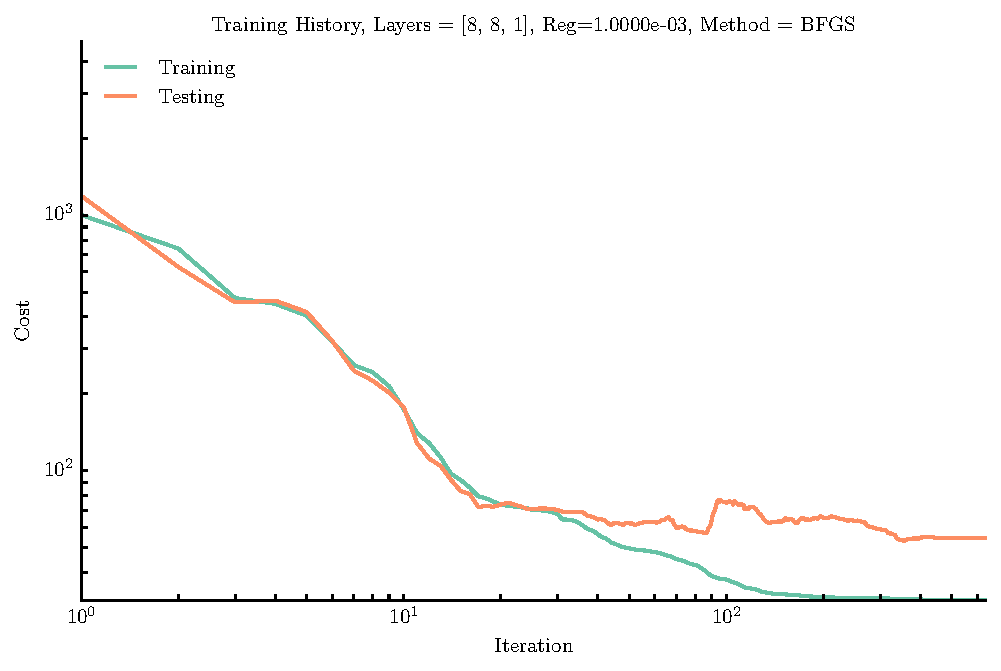
\includegraphics[width=\textwidth]{costsnnco.pdf}
\caption{The cost function history for training a FFNN on the GEOS-Chem CTM data.}
\label{fig:costCF}
\end{figure}

\begin{figure}[!htb]
\centering
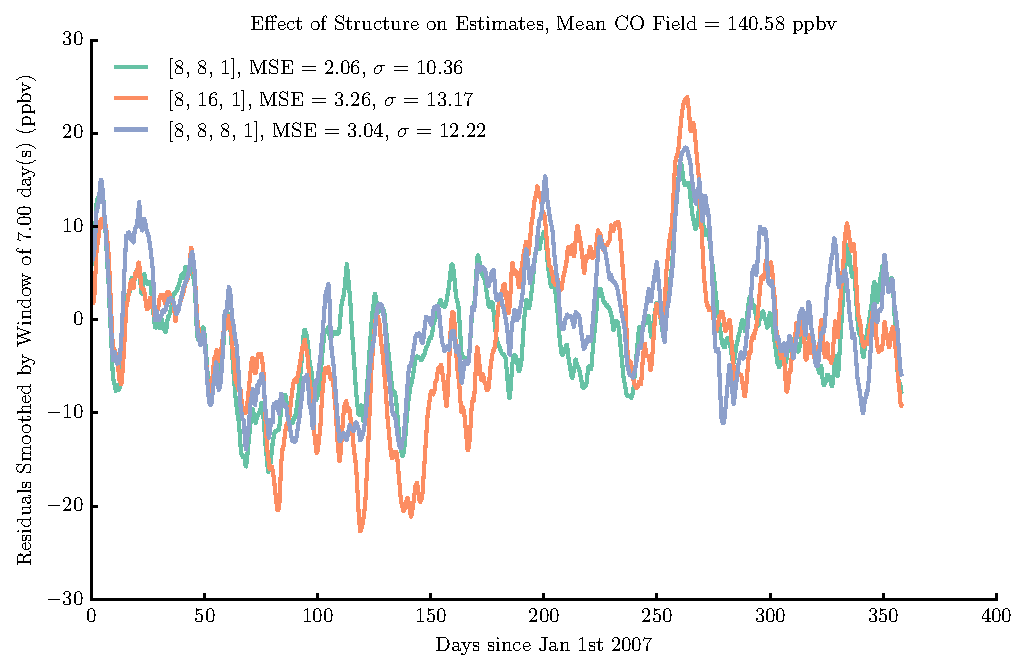
\includegraphics[width=\textwidth]{residuals_window_168.pdf}
\caption{A plot of residual data between the GEOS model and multiple neural network fits. Larger architectures do not necessarily provide proportionate improvements to the model.}
\label{fig:nncoR}
\end{figure}

\begin{figure}[!htb]
\centering
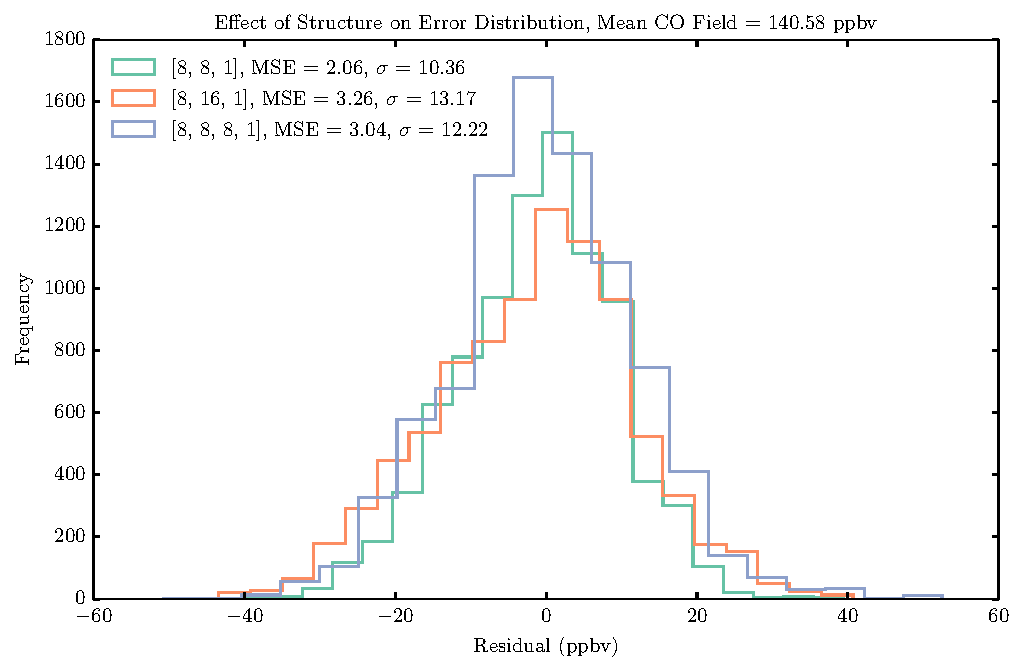
\includegraphics[width=\textwidth]{histograms.pdf}
\caption{A histogram of residuals data between the GEOS model and multiple neural network fits.}
\label{fig:nncoH}
\end{figure}

\begin{figure}[!htb]
\centering
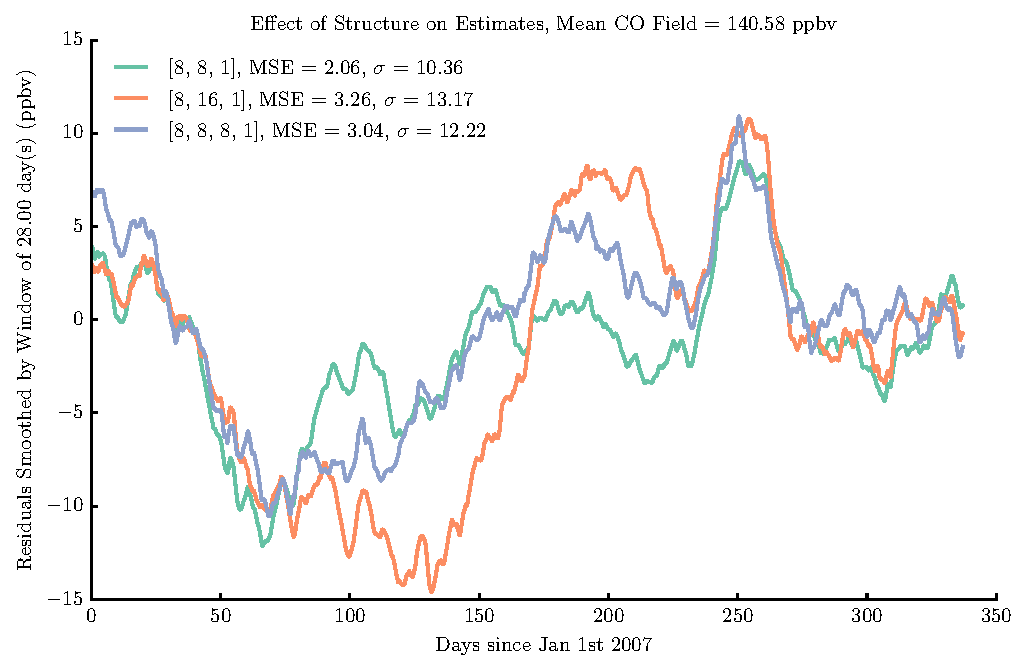
\includegraphics[width=\textwidth]{residuals_window_672.pdf}
\caption{Residuals between the GEOS-Chem CTM data and network outputs. A large smoothing window shows that all three networks capture seasonal changes without major discrepancies.}
\label{fig:nnco28}
\end{figure}

\begin{figure}[!htb]
\centering
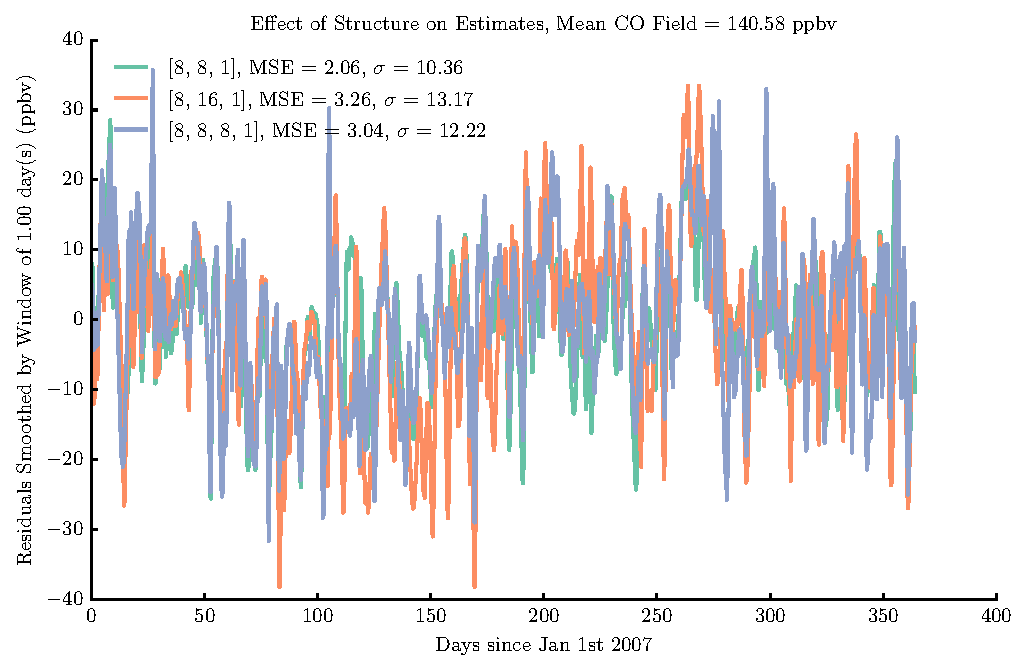
\includegraphics[width=\textwidth]{residuals_window_24.pdf}
\caption{Residuals between the GEOS-Chem CTM data and network outputs. A short smoothing window allows daily variability to leak into the data and illuminate the problem of over-fitting.}
\label{fig:nnco1}
\end{figure}

\begin{figure}[!htb]
\centering
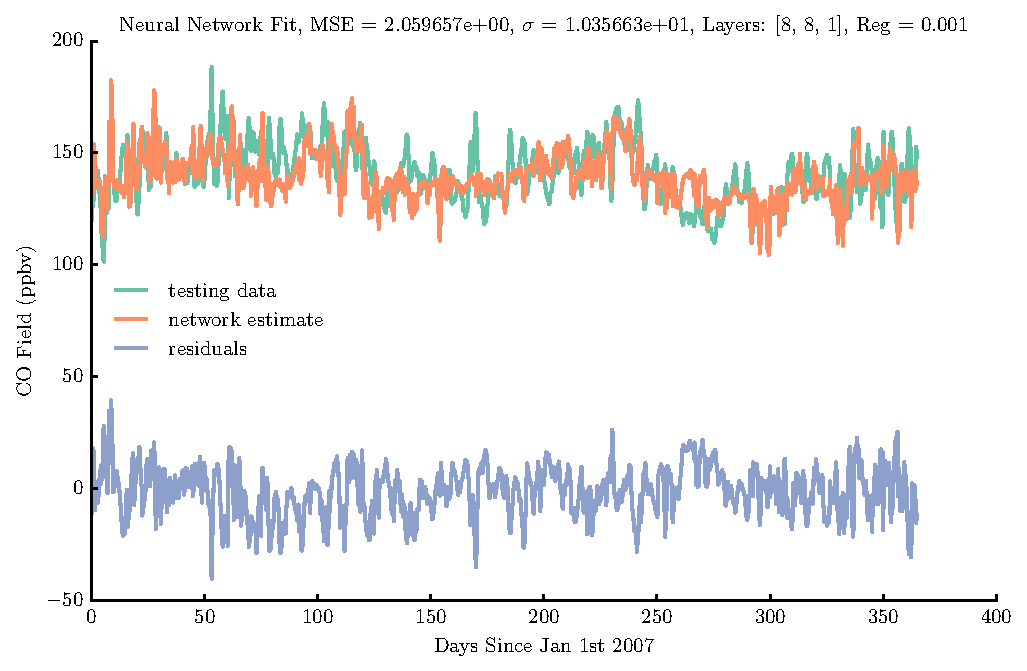
\includegraphics[width=\textwidth]{nnfield.pdf}
\caption{The raw fit of the testing data. Note the errors during the summer season.}
\label{fig:nn}
\end{figure}

\section{Conclusions and Future Work}

The statistical approach taken in these experiments have proved to be an advantageous way of modeling CO concentrations. Accurate models were constructed given short training times, small architectures, and little preprocessing of data. It is clear that given more computational resources, neural networks will be a valuable tool to use alongside modern data assimilation techniques. The next problem is one of scale. The data set is currently one dimensional in each attribute. The total GEOS-Chem CTM dataset is multivariate and of very high dimension. In order to extend this analysis to whole map modeling, efficient methods of dimension reduction must be investigated. N-way methods of tensor factorization will be considered to reduce the number of dimensions but also to retain correlation information in both spatial and temporal domains. There has been recent interest to apply convolutional neural networks to high dimensional spatial data and to use recurrent neural networks for modeling time series data. It would seem plausible then, to combine the two architectures to attack problems with both spatial and temporal correlations. Lastly, more efficient ways of training will be considered to deal with larger sets of data, as training on one year may not be enough to quantity large scale temporal activity in the data. Weight dropout, simulated annealing, and genetic algorithms will all be considered to help reach global minima in spaces that not convex and of very large size.